\documentclass{article}
\usepackage[utf8]{inputenc}

% below are a bunch of useful packages, it doesn't cost anything to include them all so you might as well
\usepackage{amsmath}		% lets you input equations in math mode
\usepackage{graphicx}		% lets you include images
\usepackage{enumerate}		% lets you make lists
\usepackage{hyperref}		% lets you make links
\usepackage{subcaption}     % if you want to use subcaptions
\usepackage[all]{hypcap}	% makes links refer to figures and not captions
\usepackage{relsize}		% lets you use relative font sizes
\usepackage{caption}        % lets you add captions
\usepackage{array}          % lets you specify table column widths
\usepackage[margin=1in, paperwidth=8.5in, paperheight=11in]{geometry} % I'll bet you can figure this one out

\title{Hardware Matrix Multiplication}
\author{Benji Pugh}
\date{December 2021}
\begin{document}

\maketitle

\section{Introduction}
Matrix operations are at the core of 3d graphics, computer vision, and machine learning. In the specific case of 3d graphics, objects can be represented as coordinates in space, and if we represent these points as vectors we can perform matrix transformations on the points to rotate, scale, translate, and project the object.

\section{Context}
Because I am particularly focusing on the hardware surrounding 3d graphics, I chose to implement a four dimensional Matrix-Vector multiplication. The reason this is four dimensional and not three is because we need to be able to perform any affine transformation (such as translation, scaling, rotation) in the three spatial dimensions, requiring us to use homogeneous coordinates (coordinates used in projective geometry) which contain a fourth component [1].

Another particularly useful use of matrix operations are in machine learning. For example, neural networks require many matrix multiplications for the forward pass of data through the network as well as in the process of backpropagation to train the network. These operations generally deal with N-dimensional arrays, meaning that this implementation of matrix multiplication is not particularly useful for machine learning, however similar concepts can be expanded to cover N-dimensional matrix operations.

Because they often deal with large quantities of data, applications of matrix math are particularly useful to optimize with peripheral devices to a CPU, the most common being GPUs which handle.

\section{Implementation}
\subsection{Specification}
I will be implementing Matrix-Vector multiplication in row-major form, which takes the following form:
\begin{equation}
    A_{4\times4} \times{} x_{4\times1} = y_{4\times1}
\end{equation}
Which represents:
\begin{equation}
A_{4\times4} \times{} x_{4\times1} =
    \left[ {\begin{array}{cccc}
    a_{00} & a_{01} & a_{02} & a_{03} \\
    a_{10} & a_{11} & a_{12} & a_{13} \\
    a_{20} & a_{21} & a_{22} & a_{23} \\
    a_{30} & a_{31} & a_{32} & a_{33} \\
  \end{array} } \right] \left[ {\begin{array}{c}
    x_{0} \\
    x_{1} \\
    x_{2} \\
    x_{3} \\
  \end{array} } \right]
  \end{equation}
  \begin{equation}
  y_{4\times1}
  = \left[ {\begin{array}{c}
    a_{00}\times{}x_0 + a_{01}\times{}x_1 + a_{02}\times{}x_2 + a_{03}\times{}x_3 \\
    a_{10}\times{}x_0 + a_{11}\times{}x_1 + a_{12}\times{}x_2 + a_{13}\times{}x_3 \\
    a_{20}\times{}x_0 + a_{21}\times{}x_1 + a_{22}\times{}x_2 + a_{23}\times{}x_3 \\
    a_{30}\times{}x_0 + a_{31}\times{}x_1 + a_{32}\times{}x_2 + a_{33}\times{}x_3 \\
  \end{array} } \right]
\end{equation}
\subsection{Fully Combinational Method}
The most basic way to implement matrix-vector multiplication in hardware is to treat the entire operation combinationally, using multipliers to multiply elements of the matrix $A_{4\times4}$ with elements of the vector $x_{4\times1}$, finally summing to produce an output.

Figure \ref{fig:comb_mult} shows a logical diagram of a fully-combinational two-dimensional matrix-vector multiplier for simplicity, however this diagram can easily be scaled to any N-dimensional matrix vector multiplication by using more multipliers and adders. 

\begin{figure}
    \centering  % this centers the image
    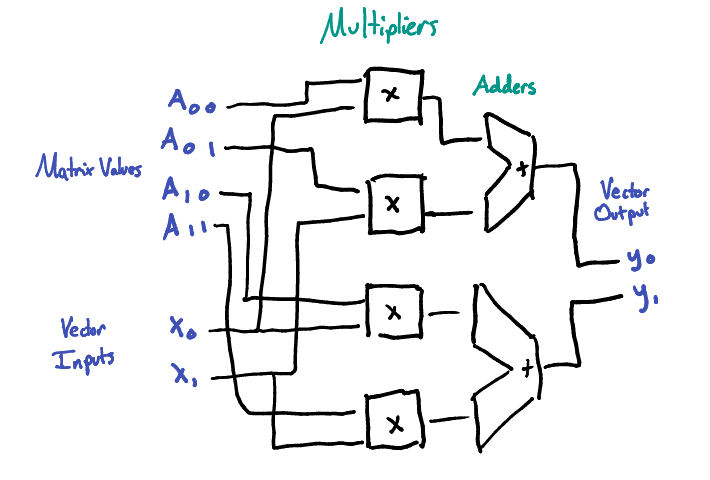
\includegraphics[width = .8\textwidth]{Combinational_Multiplier.png}
    \captionsetup{margin={0.2\textwidth,0.2\textwidth}}
    \caption{Combinational Multiplier Logic Diagram}
    \label{fig:comb_mult}
\end{figure}

This logical diagram illustrates a key problem with fully-combinational matrix operations: each dimension requires increasingly more multipliers and adders. Specifically, matrix-vector multiplication would require $N^2$ multipliers where N is the number of dimensions. This becomes unwieldy quickly and uses an enormous amount of transistors, especially when dealing with floating point numbers. An increased transistor count corresponds to longer propagation delays as well as higher cost, so this is not an ideal implementation.

\section{Sequential Method}
An improved way of handling the many arithmetic operations is to instead use only one multiplier, sequentially multiplying matrix and vector values and adding to the results.

Figure \ref{fig:seq_mult} shows a logical diagram for a sequential implementation of two dimensional matrix-vector multiplication for simplicity. The input to the multiplier consists of two multiplexers: one for the matrix values and one for the vector values. The muxes are controlled by a counter which increments through all of the matrix values, corresponding with all of the multiplication operations that need to happen. In the case of a two dimensional multiplication, the index increments through 0 to 3 (00 to 11 in binary), and for four dimensional multiplication the index increments through 0 to 15 (0000 to 1111 in binary).
\begin{figure}
    \centering  % this centers the image
    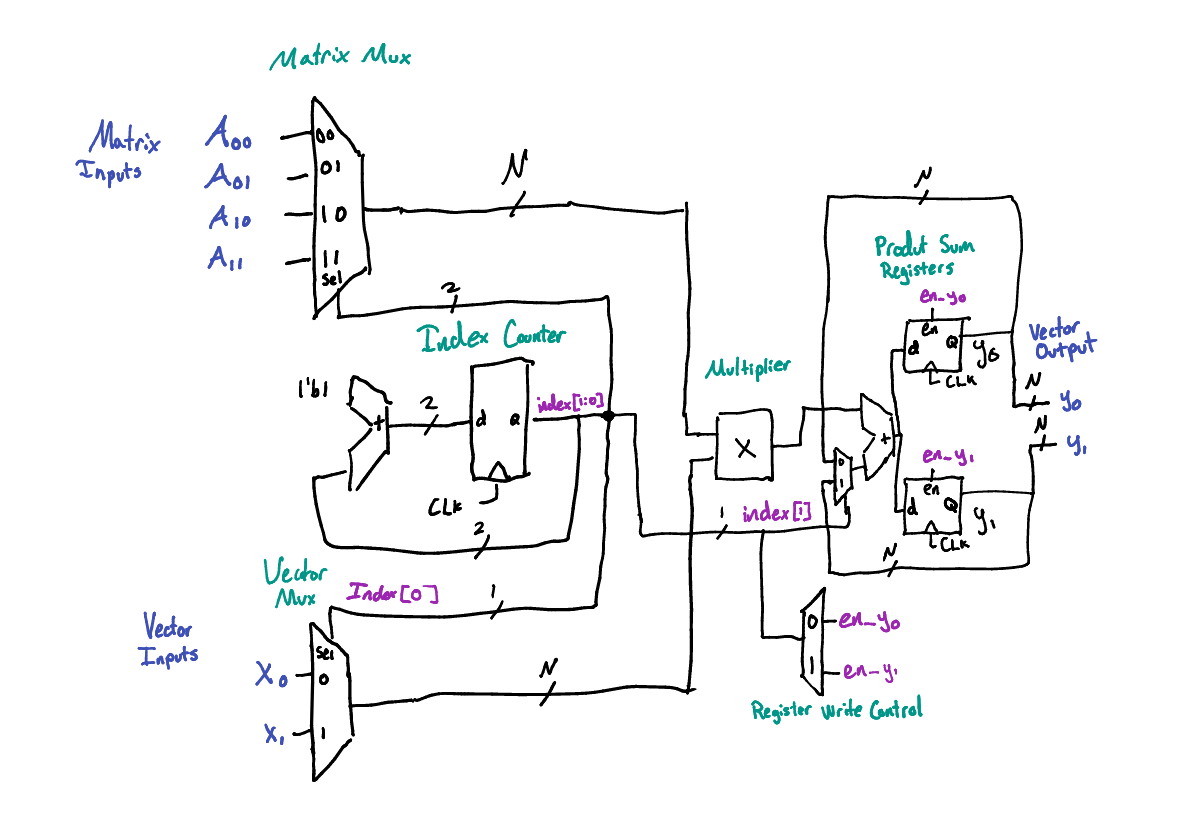
\includegraphics[width = .8\textwidth]{Sequential_Multiplier.png}
    \captionsetup{margin={0.2\textwidth,0.2\textwidth}}
    \caption{Sequential Multiplier Logic Diagram}
    \label{fig:seq_mult}
\end{figure}
The full index controls the matrix mux, while the lower half of the index controls the vector mux. This causes the matrix-vector multiplier to multiply each matrix row with the vector column. Finally, the matrix-vector product requires summing the row-column products. This is achieved by storing the results in registers, using a multiplexer and an adder to choose which result element gets added to, and using a decoder to selectively enable which register gets written to.

Figure \ref{fig:state_diag} is a state diagram of the full control for a four dimensional matrix-vector multiplier, which includes a ready/valid handshake for interfacing with the module as well as the sequential arithmetic.

\begin{figure}
    \centering  % this centers the image
    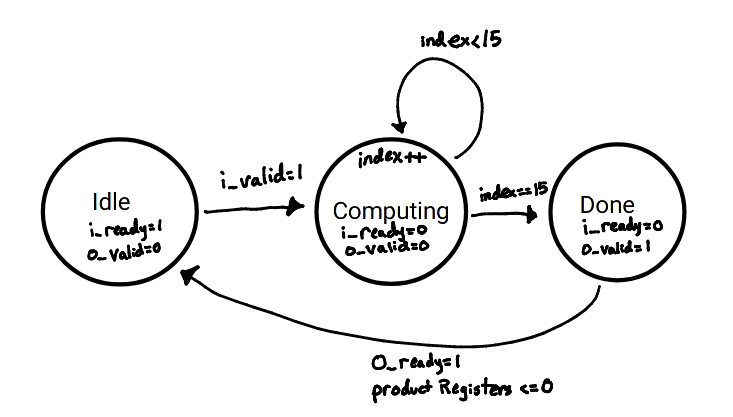
\includegraphics[width = .8\textwidth]{Handshake_State_Diagram.png}
    \captionsetup{margin={0.2\textwidth,0.2\textwidth}}
    \caption{State Diagram of Sequential Module Control}
    \label{fig:state_diag}
\end{figure}

\section{Verification}

Verifying matrix math approaches the point at which writing out full test cases in SystemVerilog becomes unwieldy due to the sheer quantity of numbers involved. To aid with the testing, therefore, I created a python script which uses NumPy to generate a testvector of both specific matrix multiplication edgecases and constrained random values.

The SystemVerilog testbench loads cases from the testvector and interfaces with the ready/valid handshake of the matrix-vector product module to compare the outputs with the values calculated in NumPy's matrix-vector multiplication.

\section{Expansion}
At it's present state, the matrix-vector product module I created is still not particularly useful. This is because it still needs quite a significant number of connections with other modules which could potentially push the limits of a FPGA fabric (all of the matrix and vector value inputs to it are currently in parallel). Expanding and reworking the module to interface over serial would assist in this module being useful in combination with other operations on data.

Alternatively, the module could be expanded to work with memory, either using Memory Mapped Registers or Direct Memory Access, making the module useful in combination with a CPU. When working with memory, pipelining data fetch actions into the matrix math becomes a major performance improvement as the module can be computing operations every cycle.

To continue the path of implementing 3d Graphics on an FPGA, this module could be used to rotate, translate, and shear 3d points as well as project them on a 2d plane. A potentially very simple path is to create a fixed-pipeline wireframe renderer for 3d points made out of set rotations, translations, and projections of the 3d points using the matrix-vector multiplication module created in this project.
\section{Citations}
\subsection{External}

[1] Resource for Understanding Matrices and 3d Graphics:

\href{https://jeffmcglynn.com/blog/2017/11/matrix-math-for-3d-computer-graphics/}{https://jeffmcglynn.com/blog/2017/11/matrix-math-for-3d-computer-graphics/}

\noindent{}[2] Details of how more robust Matrix math has been implemented on hardware:

\href{https://www.seas.ucla.edu/~baek/FPGA.pdf}{https://www.seas.ucla.edu/~baek/FPGA.pdf}

\subsection{Implemented Module}
Github Repository for the Matrix Accelerator implemented here:

\href{https://github.com/BenjiPugh/FPGA-Matrix-Accelerator}{FPGA Matrix Accelerator}
\end{document}
